\documentclass[a4paper]{report}
% begin packages %
\usepackage[utf8]{inputenc}
\usepackage[usenames,dvipsnames]{xcolor} 	
\usepackage{listings}
\usepackage{amsmath}
\usepackage{amsfonts}
\usepackage[colorlinks=true, linkcolor=black, urlcolor=blue]{hyperref}
\usepackage{todonotes}
\usepackage{listings}
\usepackage{graphicx}
\usepackage[hypcap]{caption}
\usepackage{etoolbox}
\usepackage{xifthen}
%\usepackage{}
% end packages%

% setup style %
\setcounter{secnumdepth}{3}

\newcounter{testdescr}
\newcounter{testresult}
\DeclareCaptionFormat{Test}{Test \arabic{testdescr}: #3}
\DeclareCaptionFormat{Result}{Result \arabic{testresult}: #3}
%new commands

\newcommand{\HRule}{\rule{\linewidth}{0.5mm}}

\newcommand{\addassign}[2]{
	\mathrel{+}\;\!\!\mathrel{=}
}

\newcommand\numberthis{\addtocounter{equation}{1}\tag{\theequation}}

\newcommand{\testtable}[6][ ]{
	\begin{table}[!htbp]
		%\centering
		\stepcounter{testdescr}
		\begin{tabular}{| r p{9.5 cm} |}
			\hline
			\textbf{Test id:} & \textbf{\arabic{testdescr} - #2}\\
			\hline
			\emph{Measure:}		& #3\\
			\emph{Parameters:}	& #4\\
			\emph{Values:}		& #5\\
			\emph{Motivation:}		& #6\\
			\hline
		\end{tabular}
		\captionsetup{format=Test, aboveskip=5pt}
		\caption{#2}
		\label{test:\ifstrempty{#1}{\arabic{testdescr}}{#1}}
	\end{table}
}

\newcommand{\testresult}[3][]{
	\begin{figure}[!htbp]
		\centering
		\stepcounter{testresult}
		\makebox[\textwidth][c]{\includegraphics[width=1.2\textwidth]{figure/#2}}
		\caption{#3}
		\label{result:\ifstrempty{#1}{#2}{#1}}
	\end{figure}
}


%end new commands

\begin{document}
\lstset{
	language = c++,
	tabsize = 2,
	basicstyle = \footnotesize,
	backgroundcolor = \color{White},
	commentstyle = \color{OliveGreen},
	keywordstyle = \color{Blue},
	numberstyle = \color{Red},
	stringstyle = \color{BrickRed},
	frame=single,
	morekeywords = {
		cudaMemcpy,
		cudaMalloc,
		cufftResult,
		cufftPlanMany,
		cufftHandle,
		cufftType,
		cufftCreate,
		cufftExecC2C,
		cufftComplex,
		cudaEvent,
		cudaEvent\_t,
		cudaEventCreate,
		cudaEventRecord,
		cudaEventSynchronize,
		cudaEventElapsedTime,
		__global__,
		cudaMemcpyHostToDevice,
		cudaMemcpyDeviceToHost
	}
}


\pagenumbering{roman}
% % Front page
\begin{titlepage}
\begin{center}
\textsc{\LARGE TDT4501 - Computer Science, Specialization Project}\\[0.5 cm]

\textsc{\Large Fall 2014} \\[3cm]

\HRule \\[0.5cm]
\textsc{\huge \bfseries Particle-In-Cell Codes in CUDA}\\[0.5cm]
\HRule \\[1.5cm]

\large \emph{Author}: Olav Emil Eiksund\\[0.5cm]
\large \emph{Supervisor}: Anne Cathrine Elster

\vfill
{\large \today}
\end{center}
\end{titlepage}
% Abstract
\begin{abstract}
General-purpose computing on graphics processing units, GPGPU, is a recent trend in parallel computing. With hundreds
or thousands of threads on a single device, it offers massive parallelism at a relatively low cost.

Nvidia's parallel computing environment CUDA is one of the leading GPGPU technologies. This project has
implemented a Particle-In-Cell code using CUDA and the cuFFT library. The PIC method is a technique for solving
partial differential equations, and are used to simulate the behavior of charged particles.

The different steps of the simulation algorithm have been timed for different combinations of simuilation grid resolution
and particle numerosity. Based on the results from these benchmarks we determine bottlenecks and issues with the
implementation, and give suggestions for optimizations.
\end{abstract}

%TOC and stuff
\tableofcontents
\listoffigures
%\listoftables
%
% Introduction
\chapter{Introduction}
\pagenumbering{arabic}

%%==%
This work has examined the application of GPU acceleration of \emph{Particle-In-Cell codes}, a particle simulation scheme.
Based on previous work using Pthreads, MPI and OpenMP, this work has used Nvidia's CUDA framework to parallelize the
simulation.

The particle-in-cell method consists of modeling charged particles in an electric field, with the solving of Poisson's
equation being an important step. With applications such as simulating the behavior of plasma or modeling particle
acceleration, there is an interest in performing these simulations with high accuracy, and with a good performance so as
to enable longer simulations etc.

Because of the limited resources available for this project, the scope has been more on issues encountered when developing
the simulator, rather than optimizing it for industrial or scientific use. Some questions serving as a goal for the project are:

\begin{enumerate}
	\renewcommand{\theenumi}{\alph{enumi}}
	\item Can Particle-In-Cell simulations be implemented in CUDA? Easily? \label{list:introduction-ease}
	\item Which issues are there when mapping the problem to CUDA? Which solutions or alternatives are available? \label{list:introduction-issues}
	\item Which parts of the simulation turn out to be critical paths? Can these parts of the code be improved further? \label{list:introduction-bottleneck}
\end{enumerate}

%==%
\section{Motivation}
\subsection{Why parallelize PIC codes?}
Particle-in-cell codes lends themselves reasonably well to parallelization, and the algorithm itself is quite simple,
with few steps. With few dependencies between elements, the sequential part of computation need not be to large, allowing
us to parallelize the algorithm without getting dominated by sequential code (see \ref{sec:background-speedup}).
\subsection{Why parallelize with GPGPU?}
GPGPU is a technology that makes use of a large number of slower cores to enable massive computational throughput, and
can be very cost effective compared to scaling with CPUs. Since many steps of the PIC algorithm consist of running the
same computation on all elements in a large two or three dimensional grid, GPGPU seems to be a great fit.

%==%
\section{Related Work}
A brief introduction to previous work that serves as a base for this project.

The overarching goal for the project has been to re-implement the algorithm from my advisor Anne Cathrine Elster's Ph.d.
Parallelization Issues and Particle-In-Cell Codes (Cornell, 1994) \cite{elster94} in CUDA. This work has therefore served
as an important theoretic background during development. Elster implemented a parallel PIC simulation with Pthreads
that was aimed at the distributed memory computer KSR1. Due to hardware limitations the implementation was in 2D.
The work explains the physics behind the simulation, and goes into some detail on how to optimize for performance on a
distributed shared memory machine. Elster also demonstrated how the simulation could reproduce physical phenomena such as
plasma wave oscillation when sufficient simulation parameters were chosen. While both SOR and FFT solvers \ref{sec:background-solvers}
are described and explained, the implementation made use of the FFT solver.

Jan C. Meyer \cite{meyer04} implemented PIC codes using MPI, as part of a project to compare cluster computer applicability to
supercomputer problems. The simulation is based on Elster's previous work, but uses the SOR solver instead, and rewrote
code from scratch due to problems in converting the existing work. Issues with the implementation are discussed, and it
is suggested that the implementation can be optimized quite a bit.

This was the initial goal of the masters project of Nils M. Larsgård \cite{larsgaard07}, but focus was switched to
optimizing Elster's original code. The main topic of the work is the performance of hybrid OpenMP/MPI code, and like
Meyer's code uses MPI for communication between nodes. While the FFTW library was used to improve the FFT solver
performance, OpenMP was used to accelerate the SOR solver within nodes.

%%==%
\section{Thesis Outline}
\paragraph{Introduction}
This section, an introduction to the work, and the motivation behind it.
\paragraph{Background}
Some background on the physics behind Particle-In-Cell codes, along with some insight into the two solvers used. In
addition of the recent history in parallel computing is given, with a special focus on GPGPU and CUDA.
\paragraph{Implementation}
Details about the implementation. Some known problems and issues are mentioned, as well as what can be done to improve
upon the current implementation.
\paragraph{Testing}
Various aspects of the implementation are benchmarked. Details about the testing methodology, and suggestions for further
tests to be done in the future.
\paragraph{Results}
Performance resuslts from benchmarks.
\paragraph{Discussion}
Interpretation of results and evaluation of the implementation. Existing flaws and potential for improvement is discussed.
\paragraph{Conclusion}
A summary of findings, and ideas for future work.
% Background
\chapter{Background}

% ==Particle-In-Cell Codes== %
\section{Particle-In-Cell Codes}
A technique for solving certian PDEs. Usually involves simulating particles or
fluid in a grid. Also for plasma simulations.
\paragraph{Applications}
Used for studying plasma, electrons, ions. Other applications in solid/fluid
mechanics.

% =Physics= %
\subsection{Physics}
This section should describe the physical basis for the simulation.

% Subject of simulation %
\subsubsection{Subject of simulation}
What is being modeled?
A set of particles with position velocity mass and charge. Attempting to
determine behaviour over time. Need to find force on particles. Need to
determine electric field from potential. Find potential from distribution of
charge from particles. Repeat. Simple.

Discrete in space and time. Details below.

% Equations %
\subsubsection{Discrete Model Equations}
Mention that these are the equations used in Elsters phd...
\begin{equation} \nabla^2\Phi = -\frac{\rho}{\epsilon _0} \end{equation}
\begin{equation} E = -\nabla\Phi \end{equation}
\begin{equation} \frac{dx}{dt} = v \end{equation}
\begin{equation} \frac{dv}{dt} =\frac{qE}{m} \end{equation}

\paragraph{Poissons equation}
$$ \nabla^2\Phi = -\frac{\rho}{\epsilon _0}$$
$$\frac{\partial ^2\Phi}{\partial ^2 x} + \frac{\partial^2\Phi}{\partial ^2 y} +
\frac{\partial ^2\Phi}{\partial ^2 z}= -\frac{\rho}{\epsilon _0}$$
Poissons equation: a PDE that relates the charge to the Laplacian of the potential.
\subparagraph{Describe discretization implications}

\paragraph{Electric field from Potential}
$$ E = -\nabla\Phi $$
Relates the electric field strength to the potential. The electric field
strength at a location is proportional to the gradient of the potential,
and is sampled at each grid vertex by taking the difference in each direction.

\paragraph{Electric force from the electric field}
$$ F_\text{electric} = qE $$
Electrical force is defined as the field strength $E$ times the charge $q$.

\paragraph{Acceleration, velocity - Electric force}
$$ \frac{dv}{dt} = \frac{qE}{m} $$
$$ \frac{dx}{dt} = v $$
Knowing that the acceleration of a particle $a = \frac{F}{m} = \frac{qE}{m}$,
we can estimate the velocity and position as $v = v_0 + a\cdot\Delta t$,
$p = p_0 + v\cdot\Delta t$.
\subparagraph{Describe discretization (time, space)}

% Procedure %
\subsubsection{Procedure}
\begin{enumerate}
	\item Find charge density.
	\item Solve for potential.
	\item Determine electric field from potential.
	\item Update particles.
\end{enumerate}

% ==Solvers== %
\section{Solvers}
% Boundary conditions %
\subsection{Boundary conditions}
Outline which different boundary conditions can appear, and for which ones the
different solvers are suited.

% =FFT= ++%
\subsection{FFT}
Short description of the concept behind the FFT.
\subsubsection{Fourier Transform}
Brief explanation of the math behind  the fourier transform.
\subsubsection{DFT}
How the continous transform translates to discrete applications.
\subsubsection{Cooley-Tukey FFT algorithm}
On the C-T FFT.
\subsubsection{Performance}
NlogN complexity, etc.
\subsubsection{Properties}
Aliasing etc.
\subsubsection{Applications}
Some common applications of the FFT, and reasons it is used.

% SOR %
\subsection{SOR}
\subsubsection{System of Linear Equations}
Properties of a system of linear equations. Also how this problem is represented
as one.
\subsubsection{Gauss-Seidel}
Efficient serial solver. How it translates to paralell.
\subsubsection{Over-relaxation}
How this works, and how it improves performance.
\subsubsection{Performance}
Some statistics to compare SOR to other solvers, reference point for comparison.
\subsubsection{Properties}
Tendency to "float" under certain boundary conditions, inconvergence etc.
\subsubsection{Applications}
Examples of successful application of SOR as a solver, and reasons it was used.


%% MOVE TO MOTIVATION? %%

% ==Parallel Computing== %
\section{Parallel Computing}
This section explains the motivations behind parallel programing and GPGPU in
general. It should show general characteristics of the CUDA architecture and
programming model, and show the contrast to CPU programming, mentioning both the
benefits and trade-offs, and reasons it is different.

% =Parallel computing basics %
\subsection{Parallel computing basics}
Briefly explain the essence of TDT4200, as much as is necessary to understand
the rest of the report.
\paragraph{Moore's law}
Outline regular increase in computing power as transistor density decreased.
\paragraph{Power wall, etc}
Explain why new measures had to be taken to increase performance further,
leading to increasing focus on multicore.
\paragraph{Amdahls law, Gustafsons law}
Explain what Amdahl and gustafsons laws mean for paralellization of serial
programs. How to bypass the problems by inccreasing problem size.
% ...and anything else worth mentioning. %
%%%%


% =GPGPU= %
\subsection{GPGPU}
Brief history of GPGPU, mention relationship to gustafsons law (increase
problem size at cost of processing speed). Architechture and language agnostic,
what are the benefits and costs of this approach.

% History %
\subsubsection{History}
How did GPGPU come about, and how has it developed since. Status today.

% Purpose %
\subsubsection{Purpose}
Mathematical/scientific reasons that GPGPU performs well, and why it is used.

% =CUDA= %
\subsection{CUDA}
Specifics on the cuda preogramming language/architecture. It's origin and
development since.

% Programming model %
\subsubsection{Programming model}
How to write a CUDA kernel. Why one writes a kernel. How a kernel differs from
any other funciton call.

% Architecture %
\subsubsection{Architecture}
The CUDA architecture and how it must be taken into consideration when writing
CUDA programs.
\paragraph{General}
Genral layout, function and performance of the CUDA architecture.
\paragraph{Maxwell}
Specifics for the Kepler and Maxwell generations.

% Memory %
\subsubsection{Memory}
Memory management. Different kinds of memory, allocating memory, atomic
operations etc...

% cuFFT %
\subsubsection{cuFFT}
Details on the cuFFT framework. How it is used, performance compared to FFTW...


%Previous work%
\section{Previous work}
% Implementation
\chapter{Implementation}
% ==Structure== %
Because the work this project is based on used double precision data types this is done here as well, to make sure
errors are not due to insufficient accuracy. A switch to single precision data types was left as a question to be
evaluated based on results from testing.

In contrast to the previous work however, this simulation is done in 3D, adding realism at the cost of accuracy. Adding
an additional dimension increases the number of cells by resolution in that dimension times the number of cells in the
plane. Because the memory usage and algorithm complexity increases, the resolution of each dimension will be limited.
A 3D grid of $256^3$ contains the same number of cells as a 2D grid at $4096^2$.

% % =Kernels= %
\section{Kernels}
A description of the kernels follow.

% % determineChargesFromPotential %
\subsection{determineChargesFromPotential}
The kernel determining the charge density of the mesh from particle charges. The contribution of a particle to each
vertex of its resident cell is found using trilinear interpolation, illustrated in fig. \ref{fig:trilinear}. The
distribution of a particle charge $\rho_p$ is as follows:
\begin{align*}
                \rho(i, j, k) \quad &+=\quad \frac{\rho_p }{ (h_x \cdot h_y \cdot h_z)} \cdot (h_x-a) \cdot (h_y-b) \cdot (h_z-c)\\
            \rho(i+1, j, k) \quad &+=\quad \frac {\rho_p }{ (h_x \cdot h_y \cdot h_z)} \cdot (h_x-a) \cdot b \cdot (h_z-c)         \\
            \rho(i, j+1, k) \quad &+=\quad \frac {\rho_p }{ (h_x \cdot h_y \cdot h_z)} \cdot a \cdot (h_y-b) \cdot (h_z-c)         \\
       \rho(i+1, j+1, k) \quad &+=\quad \frac{\rho_p }{ (h_x \cdot h_y \cdot h_z)} \cdot a \cdot b \cdot (h_z-c)                   \\
           \rho(i, j, k+1) \quad &+=\quad \frac{\rho_p }{ (h_x \cdot h_y \cdot h_z)} \cdot (h_x-a) \cdot (h_y-b) \cdot c         \\
      \rho(i+1, j, k+1) \quad &+= \quad \frac{\rho_p }{ (h_x \cdot h_y \cdot h_z)} \cdot (h_x-a) \cdot b \cdot c                   \\
      \rho(i, j+1, k+1) \quad &+= \quad \frac{\rho_p }{ (h_x \cdot h_y \cdot h_z)} \cdot a \cdot (h_y-b) \cdot c                   \\
 \rho(i+1, j+1, k+1) \quad &+= \quad \frac{\rho_p }{ (h_x \cdot h_y \cdot h_z)} \cdot a \cdot b \cdot c
\end{align*}
As can be seen, the contribution for a vertex is proportional to its distance to the particle compared to the other
vertices, the closest one receives the most charge and all contributions sums to $\rho_p$. Visualized in figure \ref{fig:trilinear},
dividing the cells along the interpolation lines, the contribution of a vertex is proportional to the volume of the
opposite sub-prism. We can see that the variable terms of the equations above give the volume, for instance
$\rho(i+1, j+1, k+1)$ has the term $a\cdot b\cdot c$ which is the volume of the prism in the opposite corner.

The kernel as is does not use shared memory to reduce memory latency, and it relies on slow atomic operations to avoid
write conflicts.

\begin{figure}
	\centering
	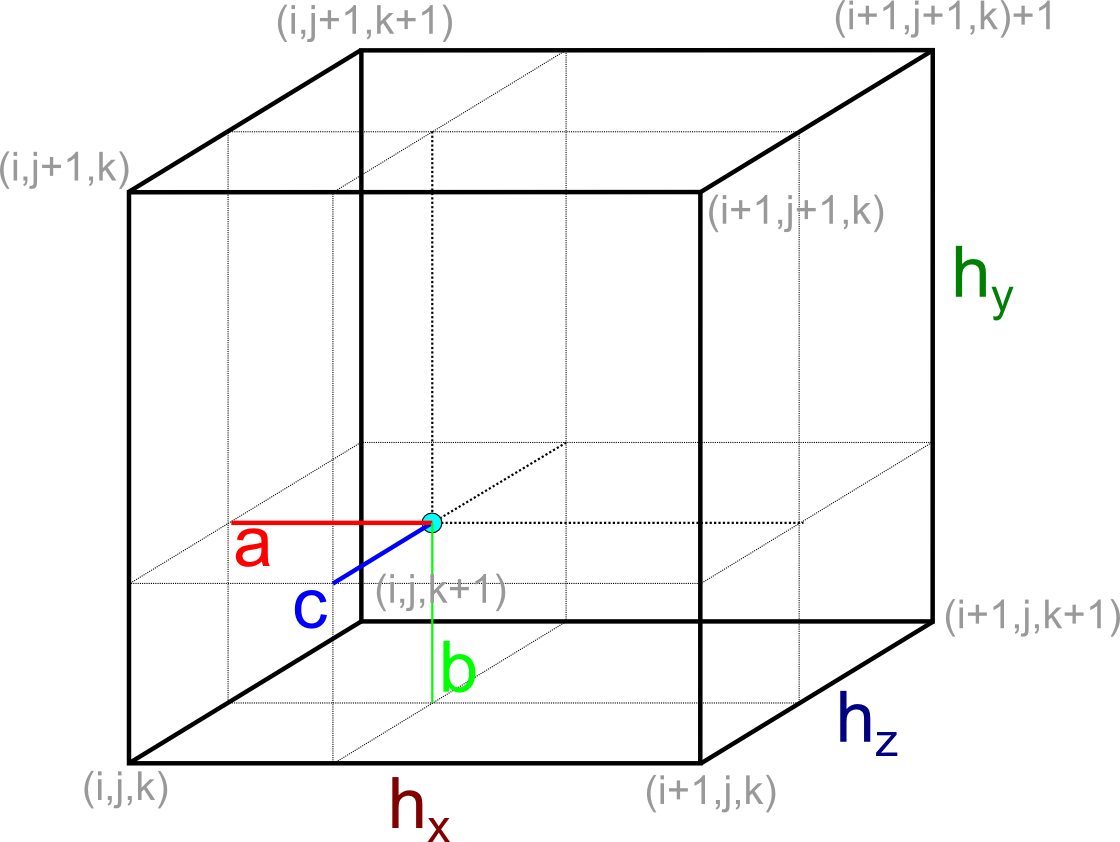
\includegraphics[width=0.8\textwidth]{figure/trilinear}
	\caption{Trilinear interpolation of particles with mesh vertices.}
	\label{fig:trilinear}
\end{figure}

% % electricFieldFromPotential %
\subsection{electricFieldFromPotential}
The electric field strength at a point is approximated as the difference in potential between it's neighbors, measured
separately in each dimension.
\begin{align*}
	E_x &= \Phi_{i+1} - \Phi_{i-1}\\
	E_y &= \Phi_{j+1} - \Phi_{j-1}\\
	E_z &= \Phi_{k+1} - \Phi_{k-1}
\end{align*}
The electric field is therefore stored as a vector at each point in the grid (array of structures).

\paragraph{electricFieldAtPoint} is a device helper function for doing trilinear interpolation of the electric field strength at some floating point
position. Similarly to the charge density calculations, field strength at a position is accumulated from cell vertices,
with contribution from each one proportional to the distance to it.

% % updateParticles %
\subsection{updateParticles}
\begin{lstlisting}
	ax = p.electricfield.x * cfg.charge_by_mass;
	prev = (1 - cfg.drag * cfg.ts);
	p.velocity.x = p.velocity.x * prev + ax * cfg.ts;
	p.position.x += p.velocity.x * cfg.ts;
\end{lstlisting}
The particle update kernel first finds the field electrical field strength at the particle's position using the helper
function electricFieldAtPoint, and then the acceleration using $a_p=\frac{F_e}{m_p} = \frac{E \cdot q_p}{m_p}$. Velocity and position
is updated through a leap frog method, where there is a $^{\Delta t}\!/_2$ delay between velocity and position updates.
$$ v^{n+ ^1\!/_2 } = v^{n+ ^1\!/_2 } + a^n \cdot \Delta t $$
$$ p^{n+1} = p^n + v^n \cdot \Delta t $$
The result is that a position update uses a velocity value that lies between the two points in time, an "average" value,
and similarly for velocity updates.


% =cuFFT= %
\section{cuFFT}
The FFT-based solver uses the cuFFT library, and this section will therefore focus on usage rather than implementation.

\subsection{FFT setup}
To run an FFT a plan has to be set up first, and stored using a cufftHandle. For single transforms with simple data
layouts the cufftPlan\#d() functions provide a simple interface for 1D, 2D and 3D transforms, while more complex setups
may need to use cufftPlanMany(). This function allows input and output  to be batched and strided data. All plans
specify the data types of the transform with options of \emph{real-to-complex}, \emph{complex-to-real}(implicitly an
inverse transform), or \emph{complex-to-complex}, and single or double precision. R stands for real, C for complex,
while D and Z are the same only for double precision.
\begin{lstlisting}
//cufftPlanMany signature
cufftResult cufftPlanMany(
	cufftHandle *plan,// Pointer to the plan
	int rank,					// dimensionality, (1, 2 or 3)
	int *n,						// n[i] = size of dimension i
	int *inembed,			// Size of dimensions in storage
	int istride,			// Distance between elements in inner dimension
	int idist,				// Distance between first elements in a batch
	int *onembed,			// Same as the above but for output
	int ostride,			// ...
	int odist,				// ...
	cufftType type,		// real or complex, single or double precision
	int batch					// multiple transforms with one call
);
\end{lstlisting}

\subsection{FFT call}
After the plan has been created, the transform can be executed using cufftExecX2X(). X2X may be either R2C, C2R, C2C,
D2Z, Z2D, Z2Z and must match the type parameter of the plan. In addition to the plan generated using cufftPlanXX(),
pointers to input and output data must ge supplied. For C2C and Z2Z an additional direction parameter must be set. R2C
is implicitly forward, Z2D is implicitly inverse and so on.
\begin{lstlisting}
//cufftExecC2C signature
cufftResult cufftExecC2C(
	cufftHandle plan,			// Plan generated as above
	cufftComplex *idata,	// Input data pointer
	cufftComplex *odata,	// output data pointer
	int direction					// Direction (forward/inverse)
);
\end{lstlisting}
\begin{lstlisting}
// Example cufft procedure
cufftHandle plan, iplan;
cufftCreate(&plan);
cufftCreate(&iplan);
cufftPlanMany(plan, ...); // Paln the transforms
cufftPlanMany(iplan, ...);
cufftExecR2C(plan, ...); // Forward transform
// ...
// Do something in spectral domain.
// ...
cufftExecC2R(iplan, ...); // Inverse transform
\end{lstlisting}

% solve %
\paragraph{solve}
After the data has been transformed using cufft, solving the for the field is done by multiplying each value by
$^1\!/_{k^2} $, and then scaling by $ ^1\!/_{\epsilon_0} $ to get $\Phi$.

$$ \frac{1}{{\epsilon_0 \cdot \left(
	\left(\frac{(2\pi \cdot \text{i} }{ L_x}\right)^2 + \left(\frac{2\pi \cdot \text{j} }{ L_y}\right)^2 + \left(\frac{2\pi \cdot \text{k} }{ L_z}\right)^2
\right)}} $$

 In addition, we need to normalize the transformation, scaling the elements by the size of the data set, which is
 $N_x \cdot N_y \cdot N_z$. The resulting computation is then to multiply the value at (i, j, k) by
 $$ \frac{1}{{4\pi^2 \cdot \epsilon_0 \cdot N_x \cdot N_y \cdot N_z \cdot \left(\, ^{\text{i}^2}\!/_{L_x^2} +\, ^{\text{j}^2}\!/_{L_y^2} +\, ^{\text{k}^2}\!/_{L_z^2}\right)}} $$
\begin{lstlisting}
scale_factor = 1/(eps_0 * 4*pi*pi * n.x * n.y * n.z);

double scale = scale_factor /
			(i*i/(l.x*l.x) + j*j/(l.y*l.y) + k*k/(l.z*l.z));

//Complex number:
row[i].x *= scale;
row[i].y *= scale;
\end{lstlisting}

% =SOR= %
\section{SOR}
From Gauss's law we have
\begin{align*}
	\nabla^2\Phi =& \frac{\partial^2\Phi}{\partial x^2} + \frac{\partial^2\Phi}{\partial y^2} + \frac{\partial^2\Phi}{\partial z^2} = - \frac{\rho_f}{\epsilon_0}\\
\intertext{This is approximated using second order finite differences.}
	\nabla^2\Phi \approx& \frac{ \Phi_{i-1} + \Phi_{i+1} + \Phi_{j-1} + \Phi_{j+1} + \Phi_{k-1} + \Phi_{k+1} - 6\Phi_{i, j, k}}{h_x \cdot h_y \cdot h_z} = -\frac{\rho_{i, j, k}}{\epsilon_0}\\
\intertext{We solve for $\Phi_{i, j, k}$}
	\Phi_{i, j, k} =& \frac{\rho_{i, j, k}\cdot\frac{h_x h_y h_z}{\epsilon_0} + \Phi_{i-1} + \Phi_{i+1} + \Phi_{j-1} + \Phi_{j+1} + \Phi_{k-1} + \Phi_{k+1}}{6}\\
\intertext{Over-relaxed updates use}
	\Phi_{i, j, k}^{(n+1)} =& (\omega-1)\Phi_{i, j, k}^{(n)} + \omega\cdot\frac{\Phi_{i-1}^{(n)} + \Phi_{i+1}^{(n)} + \Phi_{j-1}^{(n)} + \Phi_{j+1}^{(n)} + \Phi_{k-1}^{(n)} + \Phi_{k+1}^{(n)}}{6}\\
	\Phi_{i, j, k}^{(n+1)} =& \Phi_{i, j, k}^{(n)} + \numberthis \label{eqn:sor-update}\\
	&\; \omega \cdot \left( \frac{\Phi_{i-1}^{(n)} + \Phi_{i+1}^{(n)} + \Phi_{j-1^{(n)}} + \Phi_{j+1^{(n)}} + \Phi_{k-1}^{(n)} + \Phi_{k+1}^{(n)}}{6}-\Phi_{i, j,k}^{(n)} \right) 
\end{align*}
The SOR solver builds on the red-black Jacobi method described in \ref{sec:red-black}, using over relaxation to speed up
convergence. While previous work\cite[sec.~3.3.3]{elster94}\cite[sec.~2.7.2]{larsgaard07} used five-point stencils in a 2D solver, a seven-point
stencil is used to account for the z dimension, this being a 3D solver. For this solver boundary values are set equal to
the center value ($\Phi_{i, j, k}$).

As is, the kernel is run a fixed number of times, rather than checking the error. Every iteration the kernel is run
twice, once each for red and black colored tiles, allowing in-place updates in parallel.

% SOR kernel %
\paragraph{SOR kernels}
An initSOR kernel is run first, saturating the \emph{Phi} array with the appropriate values,
$$ \Phi_{i, j, k} = \frac{\rho_{i, j, k}\cdot h_x h_y h_z}{6 \cdot \epsilon_0} $$

When the SOR kernel itself is called, the \emph{k} index is calculated as follows, in order to implement red-black
coloring:
$$k = 2 \cdot Idx.z + (i + j + flag) \% 2 $$
where flag is 0 or 1 depending on whether red or black tiles are updated. The update itself uses equation \ref{eqn:sor-update}:

\begin{lstlisting}
	tmp = (left + right + down + up + front + back)/6;
	Phi[i][j][k] = center + cfg.omega * (tmp - center);
\end{lstlisting}


% =Setup= %
\section{Setup}\label{sec:implementation-setup}
The implementation currently uses parameters set in a getConfig() function, rather than with preprocessor macros. While
this prevents the compiler from optimizing certain calculations it allows parameters to be read in at runtime,
functionality that existed in Elster's original implementation, which this one it intended to be a CUDA version of.
Parameters that can be set and their default values for testing are shown in section \ref{sec:testing-parameters}.

All device memory allocations except that for the particle array use pitched pointers to ensure data alignment, helping
ensure coalesced memory accesses when possible. While the arrays probably could be reused to save space, such an
optimization is left for further improvements. For the current version the focus has been on ease of debugging and
understandability, for which separate arrays are a better fit.

Kernel grid and block settings (specified as \lstinline|kernel<<<grid, block>>>(...)|)
are chosen to achieve 256 threads per block, with a (256, 1, 1) configuration for particle-indexing kernels, and (16, 4, 4)
for field-indexing kernels. Since the particle array is one dimensional its setting is trivial, but the choice for the
three dimensional ones need some consideration. For the sake of coalesced memory access one would want threads to access
values that are sequential in the x-dimension, so it makes sense to have a wider x dimension. But if shared memory is
used to speed up computation and we want to do a border exchange, a square grid offers the fewest $^{neighbor}\!/_{element}$ ratio,
reducing the number of transfers relative to the number of in-block computations. In the implementation a value of 16 is
chosen to ensure 128-byte alignment ($16 \cdot sizeof(double) = 128$) while maximizing the block volume.

\section{Particle tracing}\label{sec:implementation-tracing}
Particle tracing is here implemented by copying the particle array from device to host every iteration. The host has a
$(N_{iterations}+1) \cdot N_{particles} \cdot sizeof(Particle)$ array, where each particle's data is stored for each
iteration. After the simulation loop has executed this array is used to output an xml file structured as follows:
\begin{lstlisting}[language=xml]
<root n_iterations="..." n_particles="..." particle_interval="...">
	<iteration time="...">
		<particle id="...">
			<position x="..." y="..." z="..."/>
			<velocity x="..." y="..." z="..."/>
			<electric x="..." y="..." z="..."/>
		<particle>
	</iteration>
</root>
\end{lstlisting}
This file is read by a python script using matplotlib to animate the movement of the particles. As of yet this script is
sensitive to the data volume, and works best with a reduced number of updates. Because of this, and in order to reduce
the performance hit associated with transferring the particle array every iteration, an interval between particle
transfers is used, $particle\_interval$. The exact interval used depends on the resolution needed to properly trace the
particles' movements, which is a function of the testing parameters and typical particle movement speed.

Another option to reduce memory transfer latency is to instead store the array on the device, and then transfer the
whole array after execution. For small values of $N_{particles}$, where the cost of initiating a transfer (API call etc.)
is significant compared to the actual data transfer, this would likely lead to some speedup since
$$T_{init} + T_{trans}(N_{trans} \cdot N_{particles}) <N_{trans} \cdot \left(T_{init} + T_{trans}(N_{particles})\right)$$.
For large values of $N_{particles}$ however this would be less pronounced, since $T_{init} << T_{trans}(N_{particles})$.
In addition, keeping a large array stored on the device consumes memory otherwise available to increase the problem size,
thus limiting the grid resolution $n_x, n_y, n_z$ and $N_{particles}$, based on the number of iterations. To get the
best of both worlds on could store a certain number of iterations' worth of data on the device, and then transfer them,
making room for further updates on the device. By selecting a transfer frequency so that 


% Testing
\chapter{Testing}

%==%
\section{Testing methodology and motivation}
In testing the implementation the goal is to see how performance is affected by various factors. This includes testing
for different problem configurations to see which parameters have the biggest impact, and testing runtime for the
different kernels to determine which ones among them are the most demanding.
The parameters that are tested for are \emph{number of iterations} $N_{iterations}$, \emph{grid resolution in all
dimensions}$n_x, n_y \text{and} n_z$, and \emph{number of particles} $N_{particles}$.
\subsection{Procedure}
\label{sec:testing-methodology}
Kernel timing is done using the following procedure based on the example by Mark Harris from Nvidia on \href{http://devblogs.nvidia.com/parallelforall/how-implement-performance-metrics-cuda-cc/}{devblogs.nvidia.com/...}.
\begin{lstlisting}
	cudaEvent_t beginning, end;
	cudaEventCreate(&beginning);
	cudaEventCreate(&end);
	
	cudaMemcpy(...);
	
	cudaEventRecord(beginning);
	// Code that should be measured goes in here.
	kernel<<<...>>>(...);
	cudaEventRecord(end);
	
	cudaMemcpy(...);
	
	cudaEventSynchronize(end);
	float timing = 0.0f;
	cudaEventElapsedTime(&milliseconds, beginning, end);
\end{lstlisting}
The code above works in the following way: cudaEventRecord(beginning) records the time of the next event recorded, which
would be the kernel call. The next cudaEventRecord(end) records when the next cuda event occurs, which would be the
cudaMemcpy call. cudaEventSynchronize(end) blocks CPU execution until the event has been recorded, ensuring a correct
measurement. By placing the code to be measured between cudaEventRecord(beginning) and cudaEventRecord(end) we can find
$\Delta t = end - beginning$.

Other tests are timed using QueryPerformanceCounter functions provided by Windows:
\begin{lstlisting}
	_int64 t1;
	
	QueryPerformanceCounter( (LARGE_INTEGER*)&t1 );
	//
	//code to be timed goes here
	//
	_int64  t2, ldFreq;
	QueryPerformanceCounter( (LARGE_INTEGER*)&t2 );
	
	QueryPerformanceFrequency( (LARGE_INTEGER*)&ldFreq );
	double result = ((double)(t2 - t1) / (double)ldFreq) * 1000.0;
	
	//or
	
	_int64 t1;

	StartTimer(&t1);
	//
	//code to be timed goes here
	//
	double result = StopTimer(t1);
\end{lstlisting}
Helper functions called StartTimer and StopTimer are used for simplicity, and to avoid code duplication.

%%==%
\section{System configuration}
The test system configuration is given in the figures below.
\subsection{Hardware}
The relevant hardware of the test system is given in table \ref{tab:hardware}.
\begin{table}[!htbp]
\begin{sloppypar}
	\begin{tabular}{|| p{1cm} | p{5cm} | p{5cm} ||}
	\hline
		CPU:&		\href{http://ark.intel.com/products/65523}{Core i7-3770K,\newline Intel} &
			3.50GHz $\times$ 4(8) \\ \hline
		RAM:&	\href{http://www.corsair.com/en/vengeancer-16gb-dual-channel-ddr3-memory-kit-cmz16gx3m2a1600c9g}{Corsair Vengeance 16 GB} &
			2 $\times$ 8192 MB DDR3 1600MHz, 667MHz max bandwidth\\ \hline
		MB:&		\href{http://www.asus.com/Motherboards/P8Z77V_PRO/}{P8Z77-V PRO,\newline ASUStek Computer Inc.} &
			-\\ \hline
		GPU:&		\href{http://www.gigabyte.com/products/product-page.aspx?pid=4319\#ov}{Nvidia GeForce 660ti, Gigabyte OC} &
			1344 Kepler CUDA Cores, 915Mhz, 2GB GDDR5\\ \hline
		PSU:&		\href{http://www.corsair.com/en/hx-series-hx650-power-supply-650-watt-80-plus-gold-certified-modular-psu}{Corsair HX650} &
			650W\\
	\hline
	\end{tabular}
\end{sloppypar}
%\begin{sloppypar}
%	\begin{tabular}{|| p{1cm} | p{5cm} | p{5cm} ||}
%	\hline
%	Machine:& 	MSI GE60 2PE APACHE PRO & \quad \\ \hline
%	CPU:&		Intel Core i7-4710HQ &	2.50GHz $\times$ 4(8) \\ \hline
%	RAM:&	8GB & 8192 MB DDR3 1600MHz, \\ \hline
%	GPU:&		Nvidia GeForce GTX 860M & Compute capability 5.0, 640 CUDA Cores, 1020Mhz, 2GB GDDR5 2505MHz\\
%	\hline
%	\end{tabular}
%\end{sloppypar}
\caption{Hardware used in testing.}
\label{tab:hardware}
\end{table}

\subsection{Software}
Relevant software is listed in table \ref{tab:software}.
\begin{table}[!htbp]
\begin{sloppypar}
	\begin{tabular}{|| p{3.5cm} | p{8cm} ||}
	\hline
		OS:& Windows 8.1\\
		C/C++ compiler:& MS C/C++ Optimizing Compiler v17.0.60610.1\\
		CUDA Toolkit version:& 6.5\\
		CUDA compiler:& nvcc 6.5.13\\
		GeForce driver:& 344.75\\
	\hline
	\end{tabular}
\end{sloppypar}
\caption{Software used in testing.}
\label{tab:software}
\end{table}

%==%
\section{Test parameter values}
\label{sec:testing-parameters}
\subsection{Constants}
Most of the parameters remain more or less fixed across tests. This is mainly because while they affect the numerical
accuracy of the simulation, they do not affect runtime performance. The values selected for these parameters are mostly
the same as those used by Larsgård \cite{larsgaard07}.
\begin{align*}
\intertext{\textbf{Physical constants}\newline
	\textit{Value of $\pi$ used in calculations:}}
		\pi &= 3.14159265359,\\
	\intertext{\textit{Value of permittivity of free space (electric constant):}}
		\epsilon_0 &= 8.854187817 \cdot 10^{-12 } F/m,\\
	\intertext{\textit{Value of electron charge (unit charge?):}}
		e_{charge} &= -1.60217657 \cdot 10^{-19 } C,\\
	\intertext{\textit{Value of electron mass:}}
		e_{mass} &= 9.10938291 \cdot 10^{-31 } kg,\\
\intertext{\textbf{Simulation parameters}\newline
	\textit{ Simulation grid size:}}
		L_x = L_y = L_z &= 0.2 m,\\
	\intertext{\textit{Time step between iterations:}}
		\Delta t &= 1 \cdot 10^{-6 } s,\\
	\intertext{\textit{Drag term:}}
		d_{drag} &= 0,\\
\intertext{\textbf{SOR settings}\newline
	\textit{SOR relaxation factor:}}
		\omega &= 1.78,\\
	\intertext{\textit{Error threshold for convergence (currently unused, fixed nr of iterations):}}
		Err_{threshold} &= 1 \cdot 10^{-9},\\
	\intertext{\textit{Number of SOR iterations run:}}
		N_{SOR\_iterations} &= 128,\\
\intertext{\textbf{Test specific}\newline
	\textit{Grid resolution (nr of points in each direction):}}
		n_x = n_y = n_z &= \text{default: } 64,\\
	\intertext{\textit{Simulation iterations run:}}
		N_{iterations} &= \text{default: } 2048,\\
	\intertext{\textit{Number of particles simulated:}}
		N_{particles} &= \text{default: } 256
\end{align*}

\subsection{Variables}
The testing parameters are $N_iterations$, $N_{particles}$ and $n_x,y,z$. Other than for tests involving the number of
iterations only the simulation loop is timed, the duration of one iteration of the simulation. Default values are $N_{particles} = 256$
and $n_x,y,z = 64$. The FFT based solver is chosen as default.

Certain simulation settings are derived from these terms, in particular the threadPerBlock and blockPerGrid settings for
each kernel. These depends on either the grid resolution or the particle count, as shown in section \ref{sec:implementation-setup}, and
while they are not testing parameters, they will vary as part of the testing.

%==%
\section{Description of tests}
Descriptions of all tests done are given below. These include definitions of the parameters tested and their values, as
well as a brief description of the motivation behind doing the specific test.

Performance will be measured as runtime of the code being tested. Time will be measured using the procedure given in
section \ref{sec:testing-methodology} (see also \href{http://devblogs.nvidia.com/parallelforall/how-implement-performance-metrics-cuda-cc/}{devblogs.nvidia.com/}\footnote{\url{http://devblogs.nvidia.com/parallelforall/how-implement-performance-metrics-cuda-cc/}}).

\subsection{Number of iterations}
This test just shows the increase in runtime as a function of the number of iterations.This should scale linearly with
$T(N_{iterations}) = N_{iterations}\cdot T(1)$, and a deviation from this would likely indicate something being wrong, or
at least interesting.

\testtable
	[iterations2]
	{Iterations}
	{$T_{simul}(N_{iterations}) -$ Simulation time, time spent in the simulation loop.}
	{$N_{iterations} -$ Number of iterations.}
	{$N_{iterations} \in [0, 2048]$}
	{This test serves only as a confirmation that runtime increases linearly with the number of iterations.}

\subsection{Grid resolution}
The resolution of the simulation grid ais likely one of a few key factors in determining performance. While we would
usually set $n_x = n_y = n_z$ and the effect of these on simulation accuracy should be equal in theory, the way the
arrays are stored in memory is different. For instance any $n_x \in [1,16]$ would result in the same memory footprint
due to padding (here assuming elements 8 byte wide and a 128 byte alignment requirement).

\testtable
	[grid1]
	{Grid - Isotropic scaling of $n$}
	{$T(n_x = n_y = n_z) -$ Application runtime.}
	{$n_x, n_y, n_z -$ Resolution in each dimension.}
	{$n_x = n_y = n_z \in [0,256]$}
	{Several of the kernels use one thread per grid element, and this metric is an important one. Two competing effects
	makes this an interesting one; a low resolution grid means less work to be done, potentially leaving multiprocessors on the
	card idle while reducing the number of memory accesses, but a high resolution one results in fewer particles per cell,
	thus potentially reducing write conflicts from particle-based kernels. See also test \ref{test:particles2}}

\testtable
	[grid3]
	{Grid - Odd and even valued $n$}
	{$T(n_x = n_y = n_z) -$ Application runtime.}
	{$n_x, n_y, n_z -$ Resolution in each dimension.}
	{$n_x = n_y = n_z = 2\cdot k, k \in [0,128]$
	$n_x = n_y = n_z = 2\cdot k+1, k \in [0,128]$}
	{Simulation time using the FFT solver with grid sizes even and odd separated, to easier compare performance.}
	
\testtable
	[grid2]
	{Grid - Scaling of $n$ along one dimension.}
	{$T(n_x = n_y, n_z) -$ Application runtime.}
	{$n_z -$ Resolution in z dimension.}
	{$n_x = n_y \in [0, 256]$\newline
	 $n_z \in [0, 256]$}
	{Here we test the effects on performance of scaling $n$ along a single dimension, for a different configuration of the
	other two dimensions.}

\subsection{Particle count}
First a measure of the impact the number of particles has on execution time, and then we see how different particle
counts perform for different grid resolutions.
\testtable
	[particles1]
	{Particles1 - Performance impact of particle numerosity.}
	{$T(N_{particles}) -$ Application runtime.}
	{$N_{particles} -$ Number of particles.}
	{$N_{particles} \in [0, 65536]$}
	{The number of particles affect device saturation; few particles mean less work to be done, fewer competing reads/writes,
	  while a higher number of particles mean a larger number of multiprocessors will be kept busy.}

\testtable
	[particles2]
	{Particles2 - Variation of both resolution and numerosity.}
	{$T(N_{particles}, n) -$ Application runtime.}
	{$N_{particles} -$ Number of particles.\newline
	  $n_x = n_y = n_z -$ Resolution in each dimension.}
	{$N_{particles} = \in [0, 65536]$\newline
	  $n_x = n_y = n_z \in [0, 256]$}
	{It can be interesting to see how particle number and grid resolution together affect performance, such as which
	  parameter affects performance the most. Given that the complexity of several operations is $O(n_x\cdot n_y \cdot n_z \cdot N_{particles})$
	  makes it interesting to see how performance scales when both are increased.}

\subsection{Comparison}
This pair of benchmarks time a single execution of each solver for varying grid sizes. The impact the grid size has on
their performance will be interesting to see, as well as which has better performance scaling.
\testtable
	[solvers]
	{Solvers - Comparing the runtime of the solvers.}
	{$T_{solver}(Solver, n) -$ Solver execution time}
	{The type of solver used.\newline
	  $n -$ Grid resolution.}
	{Solver $-$ cuFFT-based solver, SOR-solver.\newline
	  $n \in [0, 256]$}
	{By testing both solvers for various problem sizes we can get a measure of how well they scale, as well as which of them
	  offers better performance.}
	  
\subsection{Kernel runtimes}
These test involves measuring runtime for each kernel as functions of resolution and particle count. By timing each kernel
and comparing these results with the solver results we can see where bottlenecks are, and may learn how the different
kernels behave with variations of the simulation parameters. This is useful to identify what optimizations can be made
and which kernels have the most potential.
\testtable
	[kernel]
	{Kernels - Variation of resolution and particle numerosity.}
	{$T_{kernel}(n, N_{particles}) -$ Kernel execution time.}
	{$n_x, n_y, n_z -$ Grid resolution.\newline
	  $N_{particles} -$ Number of particles.}
	{$n \in [0, 256]$\newline
	  $N_{particles} \in [0, 65536]$}
	{Examining the performance for the different kernels for various configurations of particles and resolution, we may be
	able to identify potential bottlenecks. These results may assist in explaining global results above.}

%==%
\section{Suggestions for further testing}\label{sec:testing-further}
\subsection{Solver}
It would be useful to measure which of the two solvers offer better accuracy per performance. A test here could be to
set the number of SOR iterations so both solver use the same amount of time and then compare the numerical accuracy of
the results, but to do this we need to be able to tell which solver gives the best result, knowledge I do not have at
the present.

Assuming that the FFT as an exact solver gives the correct answer, we could run both and then find a measure of the
error by taking the average of the difference between the result for each element. By plotting this measure against grid
resolution and SOR iterations we could study how these increase the accuracy of the SOR. Combining this with a plot of
performance as a function of SOR iterations and grid resolution, we could see accuracy gain compared to performance loss,
an interesting metric.

\subsection{Single precision data type}
If the implementation is extended to include an option of using single precision data, it would be useful to test the
speedup this would gain us, as well as the inevitable loss of accuracy. The results of these tests could then help
give an idea of the trade-off involved in choosing one or the other.

For the single precision implementation we would also want to run most of the tests described above. At least for the
GeForce series of GPUs, throughput for single precision operations is significantly higher than for double precision
operations, more so than the reduction in bandwidth congestion. For this reason memory latency could become even more of
a factor, potentially reducing actual speedup, and test results might paint a different picture.

\subsection{System}Other tests that could be of interest are comparisons between running the same configuration on different systems. In
particular this goes for the GPU involved. The Tesla series of GPUs have significantly better double precision capabilities
compared to the GeForce series, relative to their single precision performance. A configuration that would fit on both
systems should perform better on the Tesla because of the number of available double precision floating point units,
even taking into account core, memory and bus clock speeds.
%==%

% Results
\chapter{Results}
Uncertain whether this section is needed at all. Perhaps some benchmarking
results...
\section{Section 1}
\section{Section 2}
\section{Section 3}
% Discussion
\chapter{Discussion}
%==%
\section{Results}
Some important characteristics noted during testing were:
\begin{itemize}
	\item The main factor in determining runtime is the grid resolution.
	\item The number of particles has a comparatively small performance impact.
	\item Kernel run times are relatively constant for increasing resolution.
	\item The vast majority of the computational work is done in the solver step.
	\item Our SOR solver has a high constant factor, but runtime remains more or less constant for different grid resolutions.
	\item GPU memory size is a limiting factor as far as problem size goes, preventing grid resolution much beyond $256^3$ for
	mid-end cards, and about $512^3$ for high-end cards. Particle number also has a noticeable impact on memory usage.
\end{itemize}

That execution time of charge distribution kernel decreases with larger resolution might seem counterintuitive, but since it is
called on a per-particle basis an increase in number of grid elements will have no impact on the work load. However,
because the charge distribution kernel writes to some grid element based on the particles' position, this makes fewer
particles write to the same element. By reducing these conflicts threads no longer have to wait for access, and thus
performance is improved.

Since the kernels don't appear to scale poorly with resolution the answer must be to improve the solver's scaling. As
the implementation ensures data alignment regardless of $n_x, n_y$ and $n_z$, and cuFFT is noted to perform best for
dimensions on the form $2^a \cdot 3^b \cdot 5^c \cdot 7^d$, it seems prudent to enforce this restriction on the grid
resolution. Even for values on this form, even ones tend to perform better than odd ones, suggesting that having a power
of two as a factor is desirable.

Even so, the FFT is an $O(n\cdot log\,n)$ complexity algorithm, while the SOR is relatively unaffected by the
resolution. Since the SOR is done in-place memory is much less of a factor than for the FFT solver, and it handles large grids
much better. As an element only reads from its neighbors, there is no increase in workload per thread when the number of
elements is increased. With the number of SOR iterations fixed at 128 runtime seems almost constant at 25 ms, other than
between

While resolution is still limited by memory, a measure that mey increase performance tenfold while reducing memory
footprint is to switch from double to single precision floating point values. For the GeForce series of GPUs the number
of operations per clock cycle is significantly lower for double precision. For compute capability 5.0 128 single precision
operations compared to 1 double precision, while for 3.0 the numbers are 192 and 8 \cite[sec.~5.4.1]{cudaprog}.
In addition to freeing up memory for additional resolution, there is a marked increase in processing power, utilizing
far more of the potential of the GPU.

While this holds true for consumer-grade GPUs, the Tesla series of accelerators has far better double precision
performance, with those of compute capability 3.5 capable of running 64 double precision operations per cycle.
Though, if single precision data turns out to be sufficiently accurate, the benefit of reduced memory footprint
may still justify the trade off. An interesting test in this regard would be to compare the accuracy loss of switching to
single precision versus the gain from increasing resolution. Testing this implementation on a Tesla card would also be
interesting, given the card's double precision performance.

%==%
\section{Implementation flaws, and potential fixes}\label{sec:discussion-flaws}
Listing some of the flaws to take into account when evaluating the implementation:
\begin{itemize}
	\item No use of shared memory. Important when working with CUDA, avoiding global memory accesses by utilizing the much
	faster on-chip shared memory, this should be one of the first improvements worked on. Especially the SOR-kernel should
	gain performance this way.
	\item Kernel fusion. The update particle and distribute charge kernels are called sequentially, with no dependencies on
	the first to finish execution before starting the second, and one could easily avoid expensive API calls by fusing these
	kernels together. Looking at the performance metrics however, The performance benefit would be minimal compared to
	optimizing the solver. Whether the code becomes more or less organized by fusing them is another matter.
	\item The red-black SOR currently consists of two consecutive kernel calls with an offset of one element. While this
	makes the implementation easy to understand a way of fusing these calls should be investigated. A argument in favor of
	the current implementation is that kernel calls are a trivial way to ensure the device wide synchronization needed.
	\item Particle sorting. Currently the particles maintain order in the particle array, and the same particles are put in
	a warp together every iteration. This might be wasteful, since particles on opposite sides of the grid might execute
	together, thus leading to scattered memory access. By sorting particles so that particles close together are executed
	together, we might get coalesced memory access, or even avoid different warps reading the same data. When writing data
	in the charge distribution kernel we would like to reduce the number of writes to global memory by handling writes to
	the same element in shared memory. See Elster's original work\cite[sec.~4.4]{elster94} for more details on particle sorting.

\end{itemize}

%==%
\section{Parallelizing PIC codes for CUDA}

Overall the particle-in-cell simulation seems well suited for parallel computing. All steps can be parallelized, and
there is little time spent in sequential parts of the code. Considering Gustafson's law (sec. \ref{sec:background-speedup})
we see that one can easily increase the parallel work without scaling the serial part, thus allowing unlimited speedup
in theory. Limiting factors are of course physical memory and processor throughput.

More specifically for the CUDA architecture, the mapping of a simulation step seems intuitive. Especially the grid-based
kernels map easily, given the GPU's predisposition towards 3D coordinates and stencil based computation. An issue here
is with the pitched pointers used to ensure data alignment. Using pitched pointers means accessing data using pointer
arithmetic that produces cluttered code. While this means we have fine grained control over data location, it also
leaves more room for error, and pointer calculation was indeed a major source of bugs during development. Additionally,
if we restrict the grid dimensions to a power of two for optimal FFT performance, data alignment is already taken care
of (assuming sufficiently large dimensions), and normal arrays could be used instead. 

If we want a grid resolution larger than what is possibly on GPU memory alone there is the possibility of storing the
complete grid in host memory and transferring back and forth every iteration, but this will likely become prohibitively
expensive considering the amount of data to be transferred. Other options are upgrading to a larger GPU memory, or
adding more GPU's to the system. By storing parts of the grid on different devices we only need to transfer values on the
border between them. Communication speed between devices is still an issue, but technologies like Nvidia's \href{http://www.nvidia.com/object/nvlink.html}{NVLink}
shows potential in this regard, promising speeds of up to 5 to 12 times what we would get over the PCIe 3 bus \cite{nvlink}.
For a 2 GPU 3D FFT of size $256^3$ the speedup of using NVLink is apparently nearly 2.25 over a PCIe configuration.

That the cuFFT library is readily available is another benefit of using CUDA. In CUDA version 6.5 callback functions
were added to FFT execution calls, since one usually follows a transform with some operation on the transformed data.
This way one avoids shifting control to the CPU before running the solver kernel, and using this for both the forward
transform-solver and inverse transform-electric field pairs of kernels, we avoid two of these calls per iteration.
The cuFFT library currently only supports acceleration on two GPUs, so this limits hardware scaling somewhat if this
library is to be used. An additional limit as that the entire transform must fit in memory of the GPU's involved\cite[sec.~2.8.4]{cufft-doc}.

The SOR also translates nicely to CUDA, especially if we optimize it using shared memory. One bottleneck is the error
checking, where the current implementation instead uses a fixed number of iteration. Checking whether error is
sufficiently small for all elements requires a global maximum reduction. Since this can be expensive for a large number
of elements, finding a number of iterations that is sufficient for convergence is a preferable solution. As the amount
of work done by the kernel is relatively low, an increase in the number of iterations may well outweigh the cost of
calculating the error every iteration.

%==%
\section{Solvers}
A straightforward comparison of the solvers' performance would be unfair considering that cuFFT is a highly optimizing
library while the SOR makes no use of shared memory yet. For all grid sizes 128 and below the FFT-based solver
completely outperforms the SOR, with results for 64 and below being an order of magnitude lower. It is therefore
surprising to see that the SOR has a lower runtime for $n=256$, about half that of the FFT. In addition the SOR can be
expected to handle irregular (even prime) grid dimensions far better, and since cuFFT resorts to a slower less accurate
algorithm for large primes \cite[sec.~2.12]{cufft-doc}, a lot of the difference would be made up even for smaller grid
sizes.

If the SOR is upgraded with shared memory one should also identify the best possible configuration of elements per warp/
block. Since an element reads three values from its own row plus an element from the rows above, below, in front and
behind, a total of five rows must be read to compute a value. By letting a warp handle a single row we reduce the number of coalesced
memory access to five rows. As an example lets compare configurations of threads per warp of (8, 8, 4) and (256, 1, 1),
both handling 256 elements. (8, 8, 4) reads eight elements from $8\times 4 = 32$ rows, all of which are likely scattered across
the array. (256, 1, 1) has coalesced reads from it's own row, plus four others for a total of five. Assuming dimensions
of $256^3$ this will also make the upper middle and lower rows successive in memory, resulting in only three scattered
accesses.

Since the FFT is quite communication intensive the performance benefit of switching to single precision data types is
likely greater than for the SOR kernel, and a new comparison using an optimized SOR kernel and single precision data is
warranted. Nevertheless, both solvers seem to perform comparably for problem sizes fitting in GPU memory, and the choice
is still one of selecting the one appropriate given the boundary conditions of the problem.
% Conclusion
\chapter{Conclusion}
The following questions were posed in the introduction as a goal for the project:
\begin{enumerate}
	\renewcommand{\theenumi}{\alph{enumi}}
	\item Can the simulation be implemented in CUDA? Easily? \label{list:conclusion-ease}
	\item Which issues are there when mapping the problem to CUDA? Which solutions or alternatives are available? \label{list:conclusion-issues}
	\item Which parts of the simulation turn out to be critical paths? Can these parts of the code be improved further? \label{list:conclusion-bottleneck}
\end{enumerate}
The answer to \ref{list:conclusion-ease} is yes, it is entirely possible to implement particle simulations in CUDA. The
CUDA architecture it very well suited for three dimensional computing as a result of it's origin in computer graphics,
and with a large number of libraries available the implementation need not be to complex. Whether it is easy to
implement largely depends on ones point of view. The implementation is a relatively straightforward translation of math
to code, but indexing pitched arrays and managing indexes can be difficult, and often makes up the majority of a kernel.
The cuFFT provides a useful framework for GPU-accelerated FFTs, but requires some learning and setup to get working.
Compared to OpenCL and MPI a CUDA implementation might be easier to develop, but will be far less portable.

Issues encountered during development are mainly those common to developing for CUDA, such as ensuring coalesced memory
access, avoiding write conflicts, and minimize PCIe traffic. Issues related to programming include staying within bounds
of arrays, handling pointers correctly, and identifying sources of errors.

As might be expected the solver step of the simulation turned out to be the most compute intensive step. For cuFFT there
is only so much one can do to improve performance, but among criteria listed by Nvidia are using single precision data
types to reduce bandwidth cost, and keeping transform dimensions a multiple of low primes, ideally a power of two. For
the SOR kernel we can use shared memory to reduce memory access time, switch to single precision data types, and
identify the lowest number of iterations necessary for the solution to converge with a sufficiently low error. How to
distribute elements among warps need to be investigated to find out how to best take advantage of shared memory.

\paragraph{To conclude,} the author's opinion is that CUDA can be used to accelerate particle simulations with relatively few issues.
The performance of a simulation depends on the accuracy required, more so than for a similar simulations running on the
CPU. To get a better measure of potential speedup using CUDA, more optimization of the code is necessary, as well as a
comparison with CPU code running on similar hardware.

\section{Future Work}
As discussed, the code is not very optimized, lacking even proper use of shared memory where applicable. In addition to
this changing data types from single to double precision and fusing kernels are opportunities that should be investigate.
Algorithm wise there may be some gain in devising some clever particle sorting scheme, but impact of this appears
relatively low compared to the more critical solver performance. See section \ref{sec:discussion-flaws} for details on
suggested improvements.

The particle tracing mechanism could likely be improved to minimize performance impact, and more easily facilitate
further processing. This includes both how particles are traced during simulation and how trace data is output after
the simulation has ended (see also section \ref{sec:implementation-tracing}). Real time animation of particles and
electric field would also be interesting.

Further tests have been suggested in section \ref{sec:testing-further}, some of these assuming the performance
improvements above have been implemented.

\begin{thebibliography}{13}
	\bibitem{elster94}
		Anne C. Elster,
		"Parallelization Issues and Particle-In-Cell Codes",
		1994,
		Cornell University,
		USA
		
	\bibitem{meyer04}
		Jan C. Meyer,
		"Emerging Technologies Project: Cluster Technologies, PIC codes: Eulerian data partitioning",
		2004,
		NTNU,
		Norway
	
	\bibitem{larsgaard07}
		Nils M. Larsgård,
		"Parallelizing Particle-In-Cell Codes with OpenMP and MPI",
		2007,
		NTNU,
		Norway
	
	\bibitem{libsh}
		Intel,
		\href{http://libsh.org/about.html}{"About Sh"},
		\emph{last visited on 2 January 2015}
	
	\bibitem{top500}
		\href{http://www.top500.org/lists/2014/11/}{"November 2014"},
		TOP500 The List,
		November 2014,
		\emph{last visited 2 January 2015}
	
	\bibitem{nvidiasc14intro}
		Ian Buck, Jeff Nichols and Rob Neely,
		\href{http://on-demand.gputechconf.com/supercomputing/2014/presentation/SC401-accelerated-computing-exascale.pdf}{"GPU Acceleration: What's Next"},
		Video recording: \url{http://on-demand.gputechconf.com/supercomputing/2014/video/SC401-accelerated-computing-exascale.html},
		2014,
		Supercomputing 2014,
		Nvidia
	
	\bibitem{maxwell}
		Mark Harris,
		\href{http://devblogs.nvidia.com/parallelforall/maxwell-most-advanced-cuda-gpu-ever-made/}{"Maxwell: The Most Advanced CUDA GPU Ever Made"},
		Nvidia developer zone - Parallel Forall,
		18 September 2014,
		\emph{last visited 2 January 2015}
	
	\bibitem{nvidiaopenmp}
		Jeff Larkin,
		\href{http://openmp.org/sc13/SC13_OpenMP_and_NVIDIA.pdf}{"OpenMP and NVIDIA"},
		2013,
		Super Computing 2013,
		NVIDIA
	
	\bibitem{nvcc}
		\href{http://docs.nvidia.com/cuda/cuda-compiler-driver-nvcc/}{"NVIDIA CUDA Compiler Driver NVCC"},
		CUDA Toolkit Documentation,
		1 August 2014,
		\emph{last visited 1 January 2015}
	
	\bibitem{nvptx}
		\href{http://llvm.org/docs/NVPTXUsage.html}{"User Guide for NVPTX Back-end"},
		LLVM Compiler Infrastructure,
		29 December 2014,
		\emph{last visited 1 January 2015}
	
	\bibitem{cudaprog}
		\href{http://docs.nvidia.com/cuda/cuda-c-programming-guide/}{"CUDA C Programming Guide"},
		CUDA Toolkit Documentation,
		1 August 2014,
		\emph{last visited 2 January 2015}
	
	\bibitem{nvlink}
		\href{http://www.nvidia.com/object/nvlink.html}{"NVIDIA NVLINK HIGH-SPEED INTERCONNECT"},
		High Performance Computing,
		2014,
		\emph{last visited 2 January 2015}
	
	\bibitem{cufft-doc}
		Name,
		\href{http://docs.nvidia.com/cuda/cufft/}{"cuFFT"},
		CUDA Toolkit Documentation,
		1 August 2014,
		\emph{last visited 2 January 2015}

\end{thebibliography}
All figures have been produced by the author using Inkscape, matplotlib and Google Draw.

\end{document}
